\documentclass[a4paper,12pt]{article}

\usepackage{latexsym}

\usepackage[top=3cm, bottom=3cm, left=1.5cm, right=2cm]{geometry} 

\usepackage[spanish]{babel}

\usepackage[utf8]{inputenx}

\usepackage{graphicx}

% Para los diagramas de flujo:
\usepackage{tikz}
\usetikzlibrary{shapes,arrows,positioning}

\author{Martín Buchwald (93155) \\ Ezequiel Genender Peña (93163) \\ Jennifer Woites (93274)}

\title{75.59 Técnicas de Programación Concurrente I\\
	\textbf{Segundo Proyecto}\\
	Facultad de Ingeniería, Universidad de Buenos Aires
	\date{Cuatrimestre I, 2014}
}


\begin{document}

\maketitle
\thispagestyle{empty}
\newpage
\tableofcontents
\newpage

\section{Análisis del Problema}
El problema consiste en simular una estación de servicio, teniendo que manejar los problemas de concurrencia que puedan aparecer, utilizando las técnicas vistas en la materia. Es necesario analizar cómo sincronizar y comunicar a los distintos procesos, para que la ejecución sea \underline{correcta}.\\
Problemas de concurrencia que pueden aparecer:

\begin{itemize}
	\item Varios empleados pueden querer utilizar los surtidores al mismo tiempo (un recurso
	 limitado).
	\item El jefe debe poder saber si los empleados están todos ocupados, o hay al menos uno
	 libre.
	\item Siguiendo al punto anterior, si no hay empleados libres	 asignarle a alguno el auto,
	 mientras que al mismo tiempo puede haber un empleado que acaba de terminar su tarea.
	\item Varios empleados pueden estar libres al mismo tiempo a la espera de un auto a ser
	 atendido. Es necesario que en tal caso los empleados actuen de manera sincronizada.
	\item Varios empleados, y el administrador, querrán acceder a la caja, por lo que será
	necesario sincronizar tal acceso. Además, como el administrador tiene prioridad, en caso que
	quiera usar la caja y hubieran empleados \textit{haciendo cola}, para usarla también, el siguiente
	será igualmente el administrador.
	\item Podrían llegar autos a la estación de servicio mientras el Jefe está asignándole
	otro a un empleado. Además, es necesario que el jefe atienda primero a los clientes VIP que
	a los clientes regulares (siguiendo el orden de llegada, relativamente a cada tipo).
\end{itemize}


A su vez, es necesario determinar la condición de finalización de la simulación. Se opto por finalizar la simulación luego de que transcurrió un tiempo (en segundos). Este tiempo puede ser modificado al ser pasado como parámetro al programa.
Será necesario que la finalización sea correcta; es decir, que todos los procesos finalicen sus funciones de la manera esperada, de una u otra forma dependiendo del proceso que se trate.

\subsection{Especificación: Casos de Uso}

Los casos de uso que debe contemplar nuestro sistema, son los que se ennumeran a continuación:

\begin{enumerate}
	\item \textbf{Iniciar Simulacion}:
	\begin{itemize}
		\item Actor Principal: Usuario.
		\item Actor Secundario: Estación de Servicio.
		\item Descripción: El usuario le indica a la estación que desea empezar la simulación con
		 determinados parámetros.
	\end{itemize}
	
	\item \textbf{Finalizar Simulación}:
	\begin{itemize}
		\item Actor Principal: Actor Principal: $<$Actor Temporal$>$ \textit{Fin de simulación}.
		\item Actor Secundario: Estación de Servicio.
		\item Descripción: indica que la simulación debe terminar. Ésto desencadena el resto de las
		 finalizaciones
	\end{itemize}

\newpage
	
	\item \textbf{Comenzar Trabajo}. 
		\begin{itemize}
		\item Actor Principal: Estación de Servicio.
		\item Actor Secundario: Empleado.
		\item Descripción: la estación de servicio le indica al empleado que debe comenzar sus tareas.
	\end{itemize}
		
	\item \textbf{Tomar Surtidor}
	\begin{itemize}
		\item Actor Principal: Empleado.
		\item Actor Secundario: Surtidor
		\item Descripción: El empleado toma el surtidor para utilizar.
	\end{itemize}
	
	\item \textbf{Esperar}
	\begin{itemize}
		\item Actor Principal: Empleado o Administrador, según el caso.
		\item Descripción: El empleado o administrador deberá esperar para utilizar un recurso limitado.
	\end{itemize}
	
	\item \textbf{Cargar Nafta}
	\begin{itemize}
		\item Actor Principal: Empleado.
		\item Actor Secundario: Auto.
		\item Descripción: El Empleado llena el tanque del Auto.
	\end{itemize}			

	\item \textbf{Liberar Surtidor}
	\begin{itemize}
		\item Actor Principal: Empleado.
		\item Actor Secundario: Surtidor.
		\item Descripción: El empleado libera el surtidor para que sea utilizado por otro empleado.
	\end{itemize}	
	
	\item \textbf{Cobrar}
	\begin{itemize}
		\item Actor Principal: Empleado.
		\item Actor Secundario: Auto.
		\item Descripción: El empleado le cobra al auto lo que cuesta la carga del tanque.
	\end{itemize}	
	
	\item \textbf{Asignar Auto a Empleado}
	\begin{itemize}
		\item Actor Principal: Jefe.
		\item Actor Secundario: Empleado.
		\item Descripción: Se le asigna a un empleado el auto, en caso que no hayan empleados libres se 
		va al caso de uso \textbf{Despachar Auto}.
	\end{itemize}	
	
\newpage

	\item \textbf{Despachar auto}
	\begin{itemize}
		\item Actor Principal: Jefe.
		\item Actor Secundario: Auto.
		\item Descripción: Al no haber empleado libre, se despacha al auto.
	\end{itemize}	
	
	
	\item \textbf{Depositar monto}
	\begin{itemize}
		\item Actor Principal: Empleado.
		\item Actor Secundario: Caja.
		\item Descripción: El empleado deposita el monto cobrado al auto en la caja. En caso de ser
		 necesario tendrá que \textbf{Esperar}.
	\end{itemize}	
	
	\item \textbf{Ver caja}
	\begin{itemize}
		\item Actor Principal: Administrador.
		\item Actor Secundario: Caja.
		\item Descripción: El empleado deposita el monto cobrado al auto en la caja. En caso de ser
		 necesario tendrá que \textbf{Esperar}.
	\end{itemize}	

	\item \textbf{Finalizar Trabajo}
	\begin{itemize}
		\item Actor Primario: Estación de Servicio
		\item Actor Secundario: Administrador, Jefe y Empleados.
		\item Descripción: Una vez que la estación de servicio sabe que debe terminar la simulación,
		se le indicará a los actores secundarios que deben terminar sus tareas.
	\end{itemize}	

	
\end{enumerate}

\begin{figure}
\centering
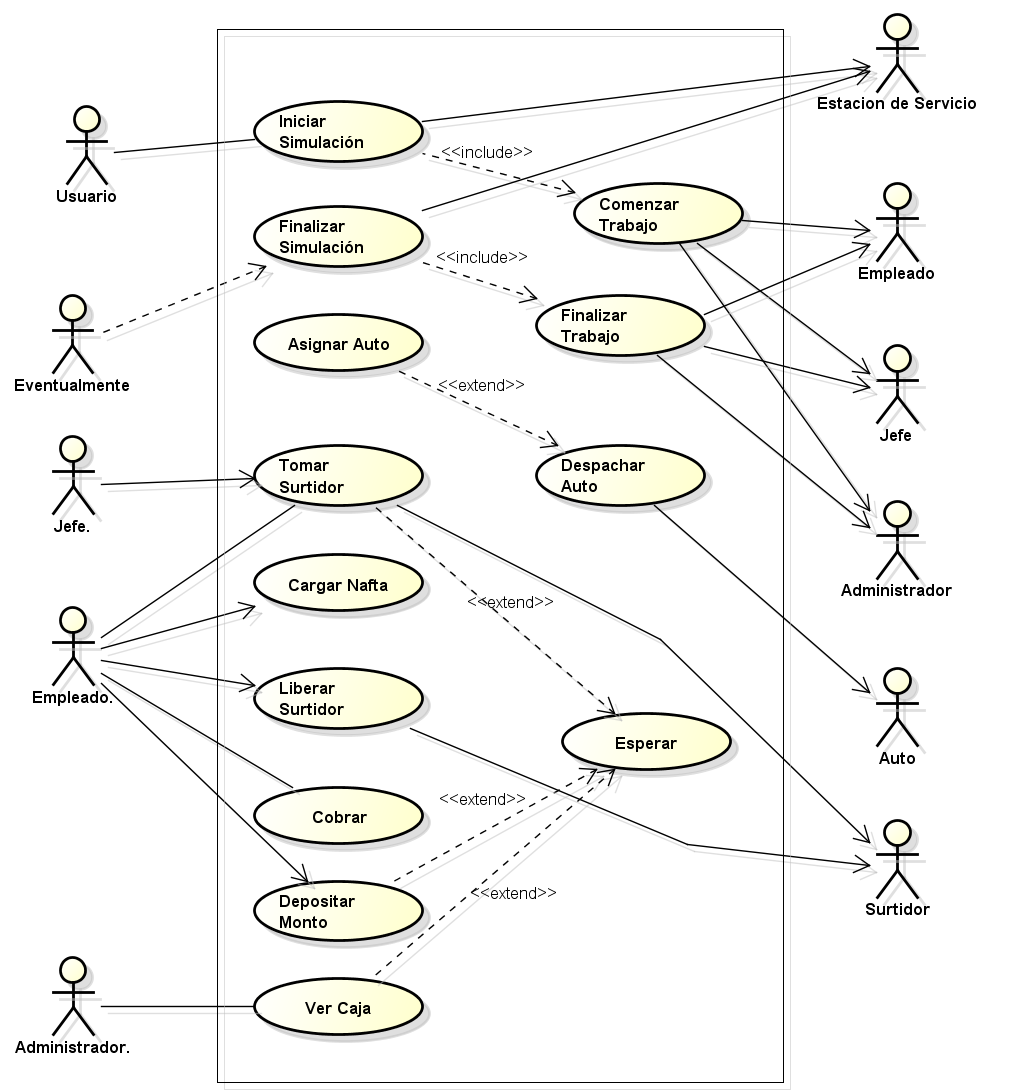
\includegraphics[scale=0.6]{Diagramas/CasosDeUso.png} 
\caption{Diagrama de Casos de Uso}
\label{fig:CasosDeUso}
\end{figure}


\newpage

\section{Resolución de Tareas}
\subsection{División de proyecto en procesos}
Luego de haber analizado el proyecto, decidimos dividirlo en los siguientes procesos:
\begin{enumerate}
\item Un proceso que simule la estación de servicio en sí. Será el principal, o dicho de otro modo, el \textit{padre} de los demás procesos del programa (teniendo que crearlos una vez que se inicia la simulación).
\item Un proceso que se encargue de generar los autos, cada un cierto tiempo aleatorio. Tales autos deberán ser enviados al Jefe para que éste los trate.
\item Un proceso que maneje al Jefe. Esto quiere decir: obtener los autos generados por el proceso anterior, y analizar si hay empleados disponibles. En caso afirmativo, debe enviarle a algún empleado el auto, y en caso negativo desestimar el 	pedido y quedar a la espera de otro auto.
\item N procesos que se encarguen de manejar a los empleados. Estos deben quedar a la espera de un auto a ser atendido, indicando su disponibilidad. Al tomar el auto, dejan de estar disponibles y proceden como está especificado en el enunciado. 
\item Un proceso que maneje al administrador, el cual irá a la caja a ver su monto cada cierto tiempo aleatorio.
\end{enumerate}


\subsection{Comunicación entre procesos}
Los procesos que se deben comunicar entre sí son:

\begin{itemize}
\item Estación de Servicio - Generador de autos: debe poder indicarle cuando debe terminar de generar autos.
\item Generador de Autos - Jefe: debe enviarle el auto que ha generado.
\item Generador de Autos - Jefe: El generador debe comunicarle al jefe, de alguna manera, que	la simulación ha terminado y por consiguiente no se generarán más autos.
\item Jefe - Empleados: debe poder conocer la disponibilidad de los empleados, para saber si enviarles el auto, o despacharlo. Por lo tanto, el dato de la cantidad de empleados disponibles es algo que deben comunicarse entre Empleados y el Jefe.
\item Jefe - Empleados: Una vez determinado que un empleado puede hacerse cargo del auto, el jefe debe enviar el auto.
\item Jefe - Empleados: El jefe debe comunicarle a los empleados, de alguna manera, que la simulación ha terminado y por consiguiente no es necesario que sigan esperando por otros autos. 
\item Empleados entre sí: los empleados deben comunicarse entre sí para poder ver cuáles surtidores están libres y cuales no. Mientras no hayan surtidores libres deberán quedarse los restantes empleados esperando a que esta situación cambie. Otro dato que deben compartir es cuáles son los surtidores libres y cuáles los ocupados.
\item Empleados entre sí, con el Administrador: Deben poder entre todos ellos acceder a la caja de manera sincronizada. Además deben compartir entre ellos el dato del monto de la caja en cada momento (puesto que los empleados lo aumentan, y el administrador lo consulta).
\item Estación de Servicio - Administrador: La estación de servicio debe poder avisarle al administrador que la simulación ha terminado, y por consiguiente debe terminar su ejecución.
\end{itemize}

\subsection{Mapeo de problemas}
Luego de analizar los problemas con los que nos encontramos, podemos hacer el siguiente mapeo con los problemas conocido de concurrencia:
\begin{itemize}
	\item La relación entre los Empleados y el Jefe puede mapearse con el problema de \textbf{Productores y Consumidores}, aunque visto desde una perspectiva un poco anti-intuitiva: los empelados producen su disponibilidad, mientras que el jefe la consume. Esto puede verse de la \textit{lectura destructiva} del jefe, dado que va reduciendo tal valor a medida que la lee, y la producción y el consumo son operaciones excluyentes, como es especificado en las características del problema.
	\item La relación entre los Empleados y el Administrador puede mapearse como el problema de \textbf{Lectores y Escritores, con prioridad para lectores}, siendo el Administrador el Lector y los Empleados los Escritores. Se puede ver que las condiciones del problema de \textbf{Lectores y Escritores} se cumplen ya que: los escritores pueden escribir de a uno a la vez; no es cierto que los lectores no puedan leer todos al mismo tiempo, dado que en este caso particular hay un único lector; además la lectura del Administrador no es destructiva.
	\item La relación entre los mismos Empleados, en función de su manejo con los surtidores, puede mapearse al problema de \textbf{Productores y Consumidores}, de la siguiente manera: los empleados van oscilando entre ser Productores y ser Consumidores. Cuando quieren obtener un surtidor, estarán consumiendo el surtidor. Cuando lo liberen, estarán permitiendo que otro empleado (o incluso él mismo) lo utilice. Básicamente, el producto en cuestión es la disponibilidad de los surtidores, que es consumida y producida por los mismos empleados.
\end{itemize}


\subsection{Mecanismos de concurrencia para la comunicación}
A continuación se comentan la comunicación que debe haber entre procesos, así como los mecanismos de concurrencia adoptados para resolver tal comunicación.
Es importante notar que cada vez que se hable de utilizar Memoria Compartida para comunicar datos entre procesos, habrá un Semáforo binario interviniendo para manejar el sincronismo de acceso a la memoria compartida. De ahora en más se deja implícito ésto, pero es de remarcada importancia no olvidar que siempre estará presente este hecho. Además, se le agrega a la memoria compartida la funcionalidad de poder incrementar el valor actual que tiene. Esto se hace porque pueden haber errores de concurrencia si primero leyéramos el dato actual, y luego se escribiese (el dato reciéntemente leido podría pasar a ser inválido). Por esto, se agrega tal funcionalidad, la cual realiza ambas operaciones, protegidas en conjunto por el semáforo incorporado a la memoria compartida. 

\subsubsection{Generador de Autos - Jefe}
Una vez iniciada la simulación, el generador de autos le irá mandando autos, cada cierto tiempo aleatorio \footnote{Se modela la llegada de autos como correspondiente a un proceso puntual de Poisson, por lo tanto, el tiempo de espera hasta que llegue un nuevo auto corresponde a una variable aleatoria de distribución exponencial, por lo que luego de enviar un auto se realiza una simulación de tal variable, para ver el tiempo de espera para crear el siguiente auto.}, y el jefe debe poder obtenerlos.
Por lo tanto, se realiza esta comunicación con un Pipe, en el cual el Generador escribe y el Jefe lee. De esta manera, el jefe puede realizar sus tareas de asignación mientras el generador le envía un nuevo auto, o incluso se logra que mientras no llegue un nuevo auto a ser atendido, el jefe quede en estado bloquedo, estado deseado dado que el Jefe no tendrá nada que hacer en esos momentos.
Al hacer uso del Pipe, se logra también que cuando el generador ya no siga generando \footnote{El proceso del Generador De Autos termina, y el Pipe queda con el fd de escritura cerrado.}, porque finalizó el tiempo de simulación, el Jefe recibe un EOF y por ello finalice su ejecución.

\subsubsection{Jefe - Empleados}
Una vez que el Jefe tiene un auto para ser atendido, debe analizar si hay empleados disponibles. Es importante notar que al Jefe no le interesa saber qué empleados están disponibles, sino cuántos (o mejor dicho, saber si tal cantidad es igual o mayor que 0).

Para poder comunicar esta información entre los empleados y el jefe, se dispone de una memoria compartida, para un simple valor entero. Cada vez que un empleado pasa a estar disponible (puesto que ya terminó con sus tareas), aumentará en 1 el valor de tal memoria (que iniciará en 0). Cuando el Jefe necesite ver si hay algún empleado disponible, verá el contenido de esa memoria compartida. Si es igual a 0, no hay ningún empleado libre actualmente, por lo que se despacha al auto, y el jefe espera a que llegue otro auto para ser atendido. Si es mayor a 0, se disminuirá en una unidad la disponibilidad (puesto que habrá un empleado menos disponible), y se le envía a los empleados el auto. 

Es muy importante notar que no pueden ser los empleados los encargados de disminuir su disponibilidad, por más que a priori suene lo más intuitivo.
Proponemos el siguiente ejemplo, siendo el empleado quien disminuye su disponibilidad: supongamos el caso de tener un único empleado, el cual se encuentra inicialmente disponible. El jefe verá que la disponibilidad será de 1 empleado, por lo que envía el auto. Supongamos también que \textit{el empleado es muy lento}, y no llega a disminuir su disponibilidad antes que el jefe vuelva a tener otro auto para atender, por lo que éste volvería a ver la disponibilidad de empleados en 1, cuando esto no es cierto. Por esta razón es importante ver que debe ser el jefe quien disminuye la disponibilidad. Otra forma de verlo es viéndolo desde el lado del análisis de mapeo a problemas conocidos de concurrencia: el jefe es el que \textit{consume} la disponibilidad de los empleados, mientras que los empleados la \textit{crean}. Evidentemente, al ser el jefe quien la consume, debe ser éste quien disminuya su valor.

Además el jefe deberá poder enviar los autos a los empleados. Se optó para ésto hacer uso de un Pipe, en el cual escribe el Jefe, y leen los Empleados. Es necesario utilizar un semáforo binario para poder sincronizar la lectura del pipe entre los N empleados.
Al hacer uso del Pipe, como se explicó en el caso Generador-Jefe, se logra que cuando el Jefe ya no vaya a enviar más autos, porque finalizó el tiempo de simulación, cada Empleado que entre a leer al pipe, reciba un EOF y por ello finalice su ejecución.


\subsubsection{Empleados entre sí}
Nos interesa que mientras hayan surtidores libres, se pueda seguir accediendo a ellos, pero una vez que no hayan surtidores libres, los empelados se queden esperando a que tal situación cambie.\\
Se utilizará un semáforo inicializado con valor M (cantidad de surtidores). A medida que cada empleado desee usar un surtidor deberá hacer \textbf{wait} del semáforo, y al dejar de usar el surtidor, se deberá hacer \textbf{signal} para que otro empleado pueda utilizarlo.

Dado que será necesario saber cuál surtidor se está tomaando en cada momento, tendremos un vector de M Memorias compartidas, de valores booleanos. Cada una de esas memorias compartidas representa a un surtidor, siendo que puede estar o no ocupado (originalmente están desocupados). Cuando un empleado quiere utilizar un surtidor, procede como fue explicado en el párrafo anterior. Luego de poder acceder a los surtidores, necesariamente habrá algún surtidor libre (puesto que pasó por el semáforo en el cual su contador está directamente relacionado con la cantidad de surtidores libres). El empleado ve surtidor por surtidor hasta encontrar uno libre. Una vez que un empleado toma el surtidor debe establecer tal surtidor como \textbf{ocupado}. Al terminar de usarlo, pasa a marcarlo como \textbf{desocupado} (y recién ahí hace el \textbf{signal} del semáforo M, para evitar problemas de concurrencia posibles).

\subsubsection{Empleados y Administrador}
Los empleados deberán, junto con el admintrador, utilizar sincronizadamente el dato del monto de la caja. Para ello se hace uso de una Memoria Compartida, de valor real (float) ya que se trata de dinero, sincronizada con su respectivo semáforo interno, como ya fue mencionado anteriormente.

Además, para poder darle prioridad al Administrador respecto de los empleados, se utiliza otro semáforo (binario, inicializado en 1) para el acceso de los empelados. De esta manera, cuando los empleados quieran usar la caja, deberán hacer wait de tal semáforo, para luego ir a utilizar la caja (que cuenta con su semáforo para sincronizar el acceso). De esta manera, Solo puede haber un empleado intentando acceder a la caja a la vez. El administrador no necesita hacer wait del anterior semáforo, pasando directamente a la caja. Por lo tanto, cuando el administrador quiera usar la caja hay dos opciones posibles: no hay nadie queriendo utilizando la caja\footnote{pasa directamente por el wait de la memoria compartida de la caja} o hay algún empleado utilizando. En el último caso, no puede haber otro empleado esperando para utilizar la caja\footnote{i.e. no hay otro empleado haciendo wait del semáforo de la memoria compartida}. De esta manera, el siguiente que utilizará la caja será necesariamente el administrador, que se adelantará a \textit{la fila de empleados} en el anterior semáforo, logrando entonces generar la prioridad de lectura buscada.

\subsubsection{Comunicación para finalizar la simulación}
Quien se encarga de terminar la simulación (y hacerle llegar tal finalización al resto de los procesos) es la Estación de Servicio (que corresponde al proceso principal).

Dado que el Administrador se ejecuta de una manera casi completamente unilateral al resto de la simulación (más allá del sincronismo con los empleados), se decide optar por enviarle una señal al proceso del administrador, el cual tendrá el \textit{signal handler} correspondiente \footnote{Se comporta seteando una variable interna del objeto signal handler para luego poder hacer el \textit{gracefull quit}}. De esta manera, la próxima vez que esté por ver la caja, verá que le habían mandado la señal de finalización, terminando exitosamente su tarea.

A su vez, optamos por informale al generador que debe terminar de generar autos por el mismo método. El generador luego de enviar su último auto verá que le enviaron una señal (puesto que tiene su respectivo \textit{signal handler}), por lo que terminará su ejecución, cerrando previamente el Pipe de envíos hacia el Jefe. A partir de aquí se generará una reacción en cadena: cuando el jefe haya leido todos los autos que hayan quedado en el pipe, leerá un \textbf{EOF}, lo cual justamente implica que el generador no generará más autos. Entonces el jefe sabrá que su tarea también ha terminado, cerrando el Pipe de comunicación con los empleados (y también hacia el Pipe hacia el Generador), y terminando su ejecución. A su vez, los empleados seguirán atendiendo los autos, pero tarde o temprano cada uno de ellos leerá el \textbf{EOF} de su propio Pipe de comunicación con el Jefe, por lo que sabrán que su tarea también ha terminado, cerrando el Pipe mencionado, y terminando su ejecución. Notar que de ésta manera todos los procesos terminan su ejecución, habiendo atendido (o despachado) todos los autos que se hubieran creado por el generador hasta haber recibido la señal de finalización.

\section{Diagramas de Comunicación entre procesos}
	En el diagrama general, se pueden observar cómo los distintos procesos se comunican entre sí, y los pasos básicos que van realizando para su normal desarrollo.
	Por simplificación del diagrama, no se muestran las señales (como SIG-PIPE por ejemplo) que se dan en caso de errores.

\begin{figure}
\centering
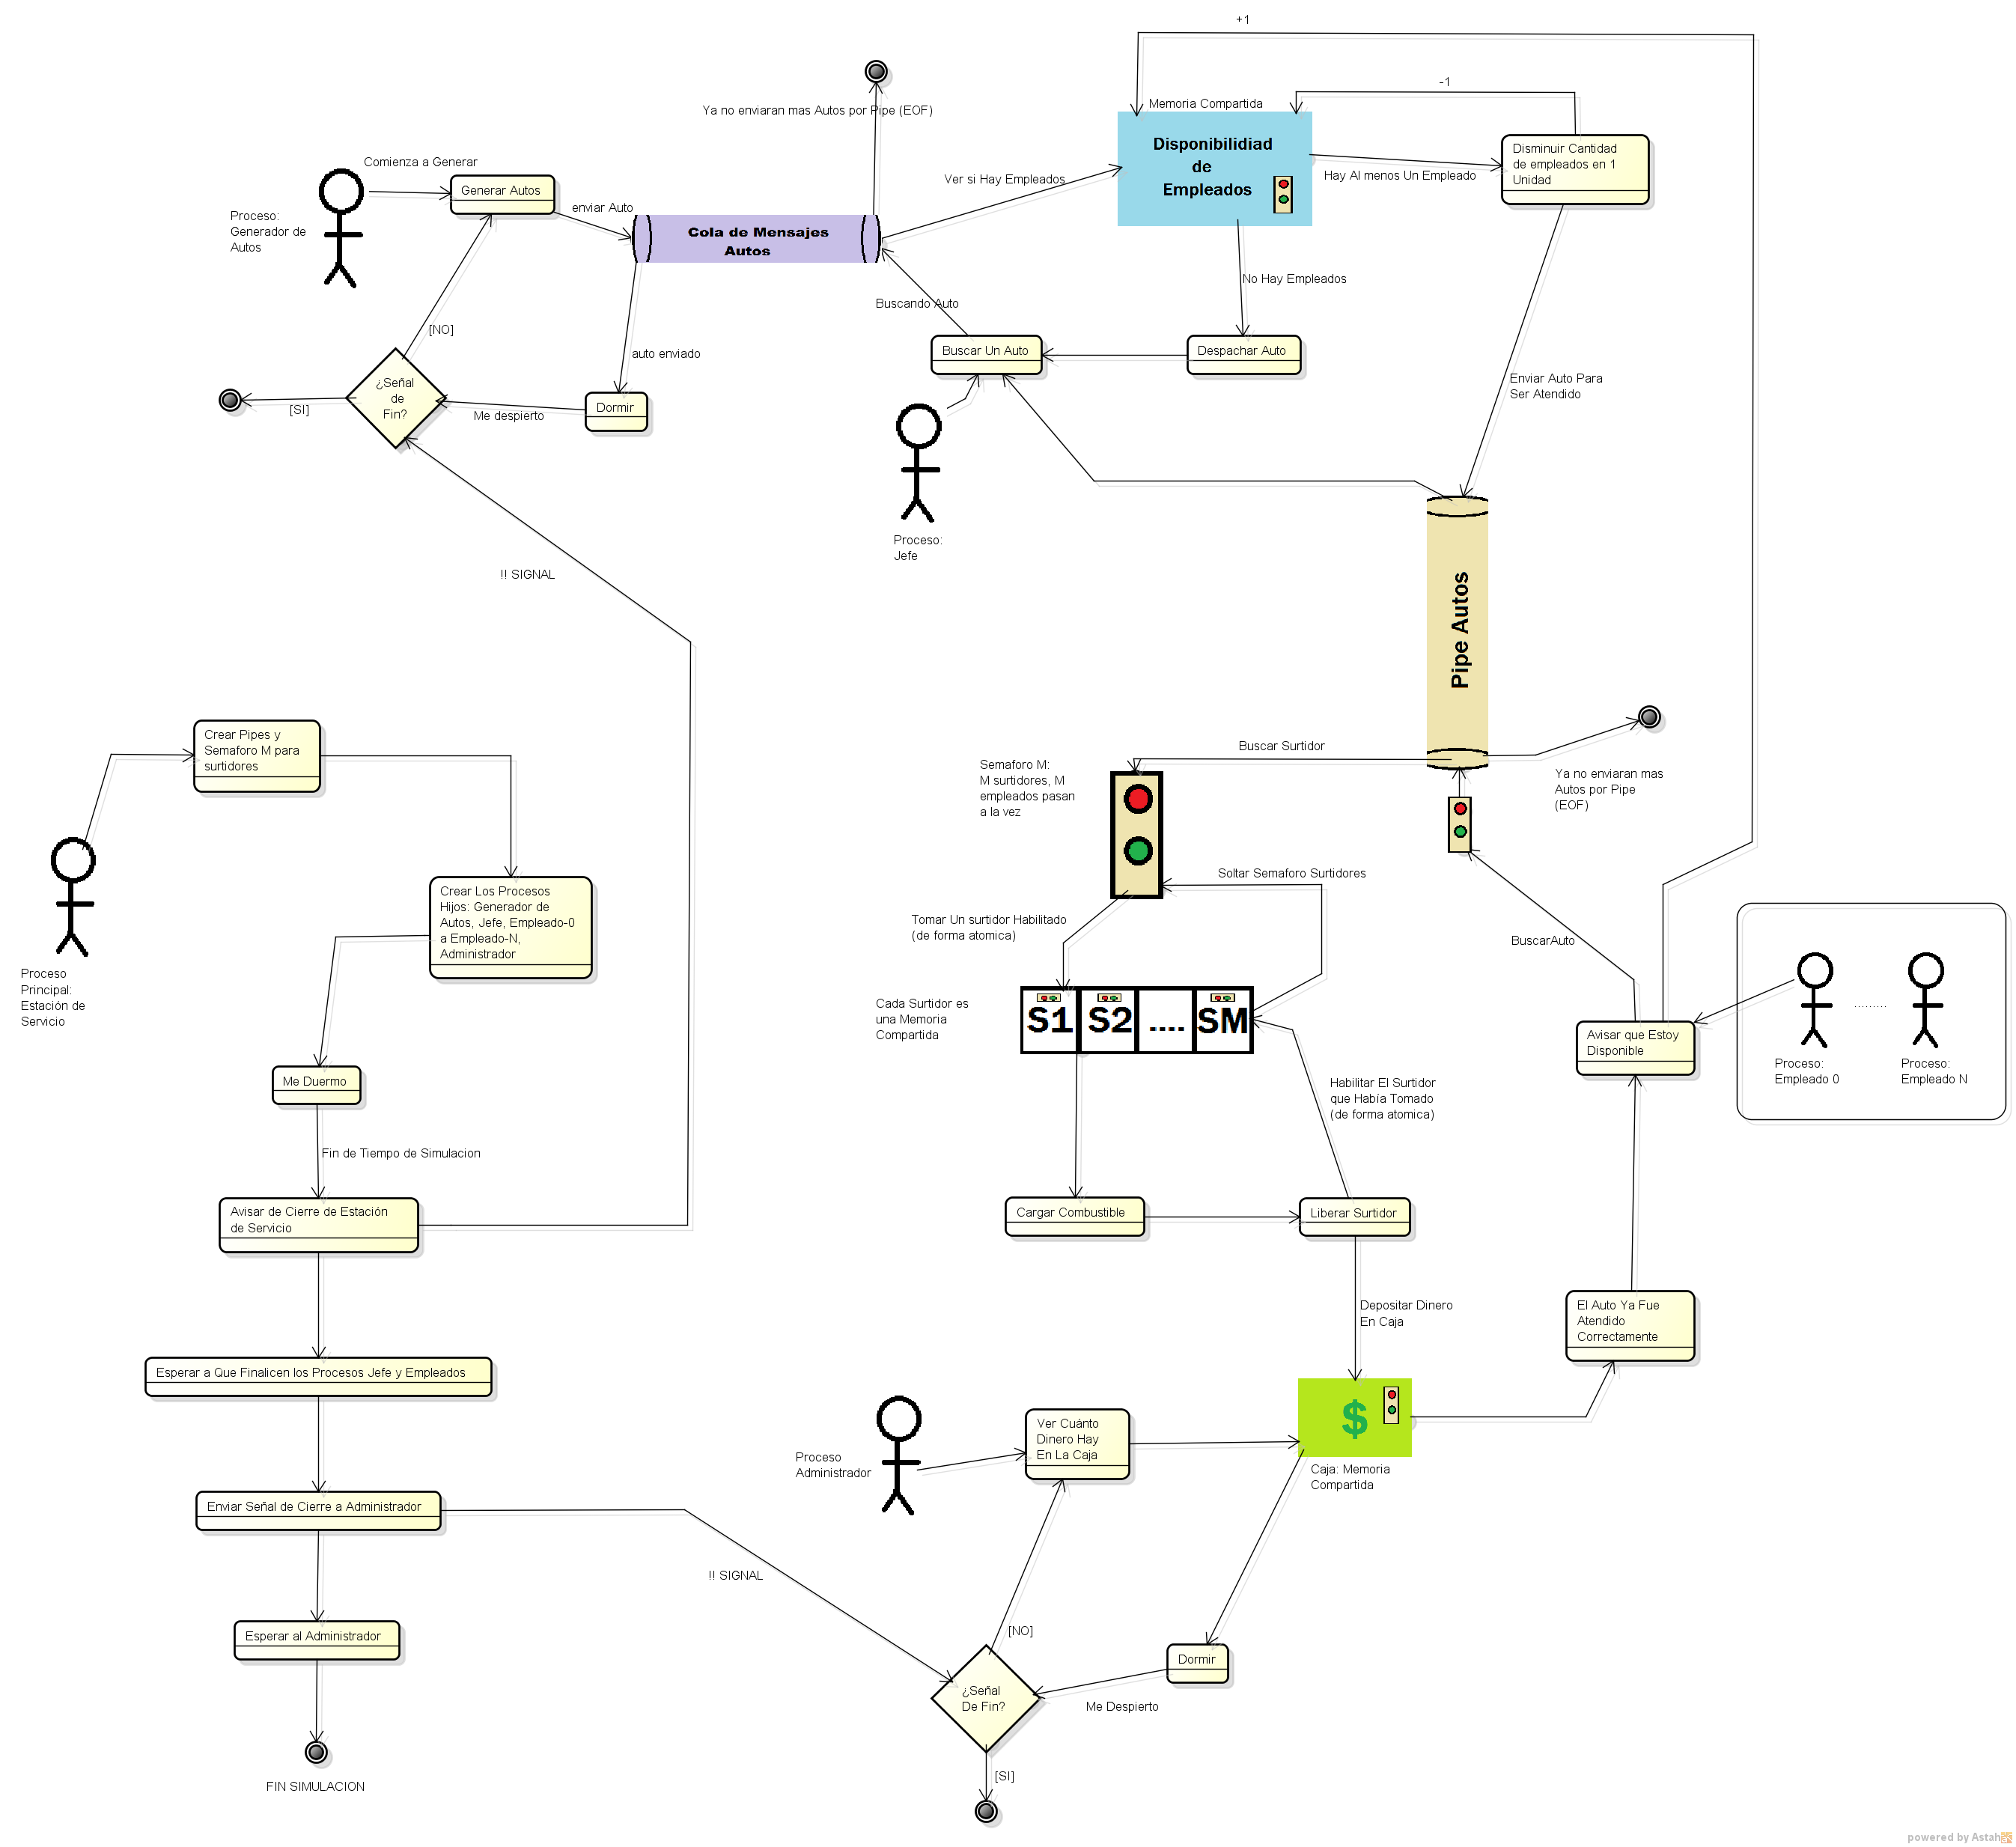
\includegraphics[width=\textwidth]{Diagramas/DiagramaFuncionamientoGeneral.png} 	
\caption{Diagrama de Funcionamiento y Comunicación General}
\label{fig:DiagramaFuncionamientoGeneral}
\end{figure}


	Podemos observar también los diagramas de comunicación entre procesos, observando la interación específica que realiza un proceso con los demás y por qué medio se realiza la misma.

\begin{figure}
\centering
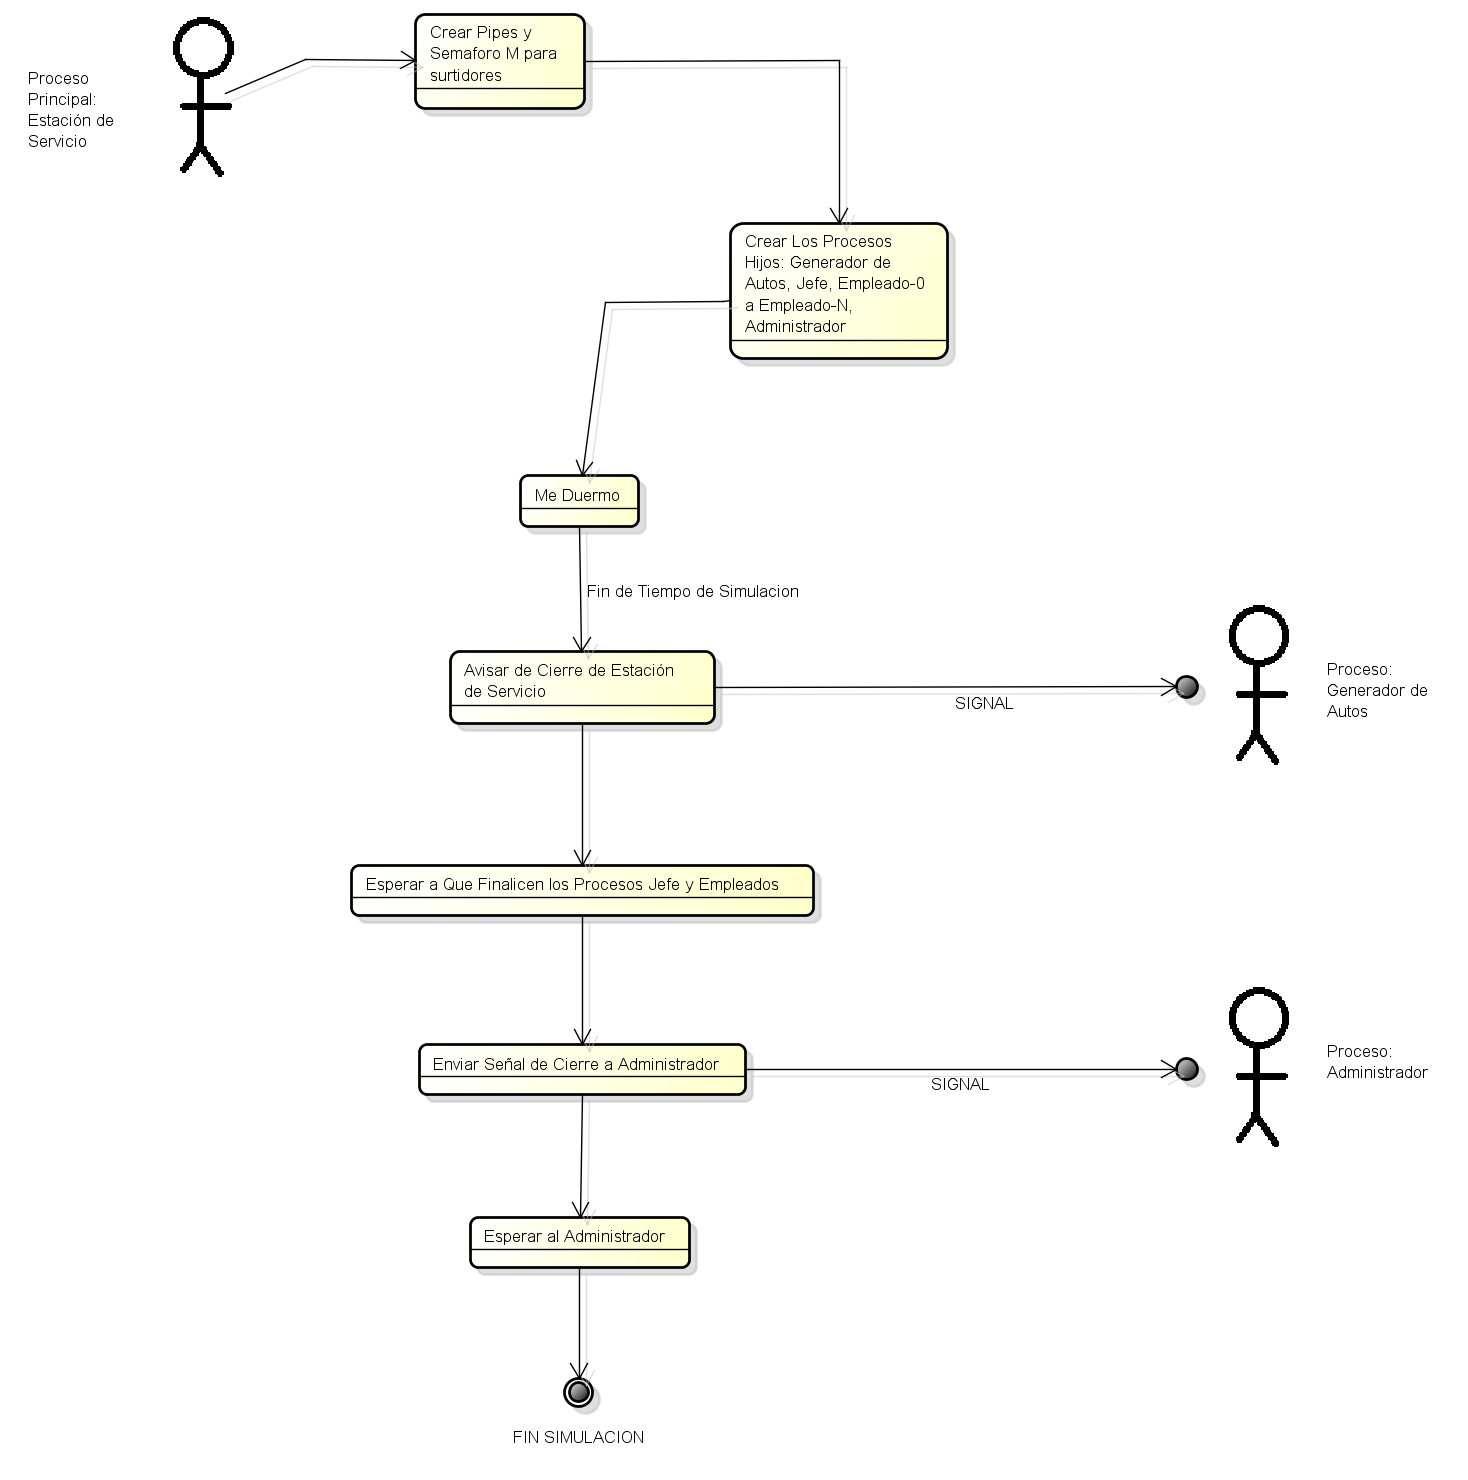
\includegraphics[scale=0.45]{Diagramas/EstacionDeServicio.png}
\caption{Diagrama de Funcionamiento y Comunicación de Estación de Servicio}
\label{fig:EstacionDeServicio}
\end{figure}	

\begin{figure}
\centering
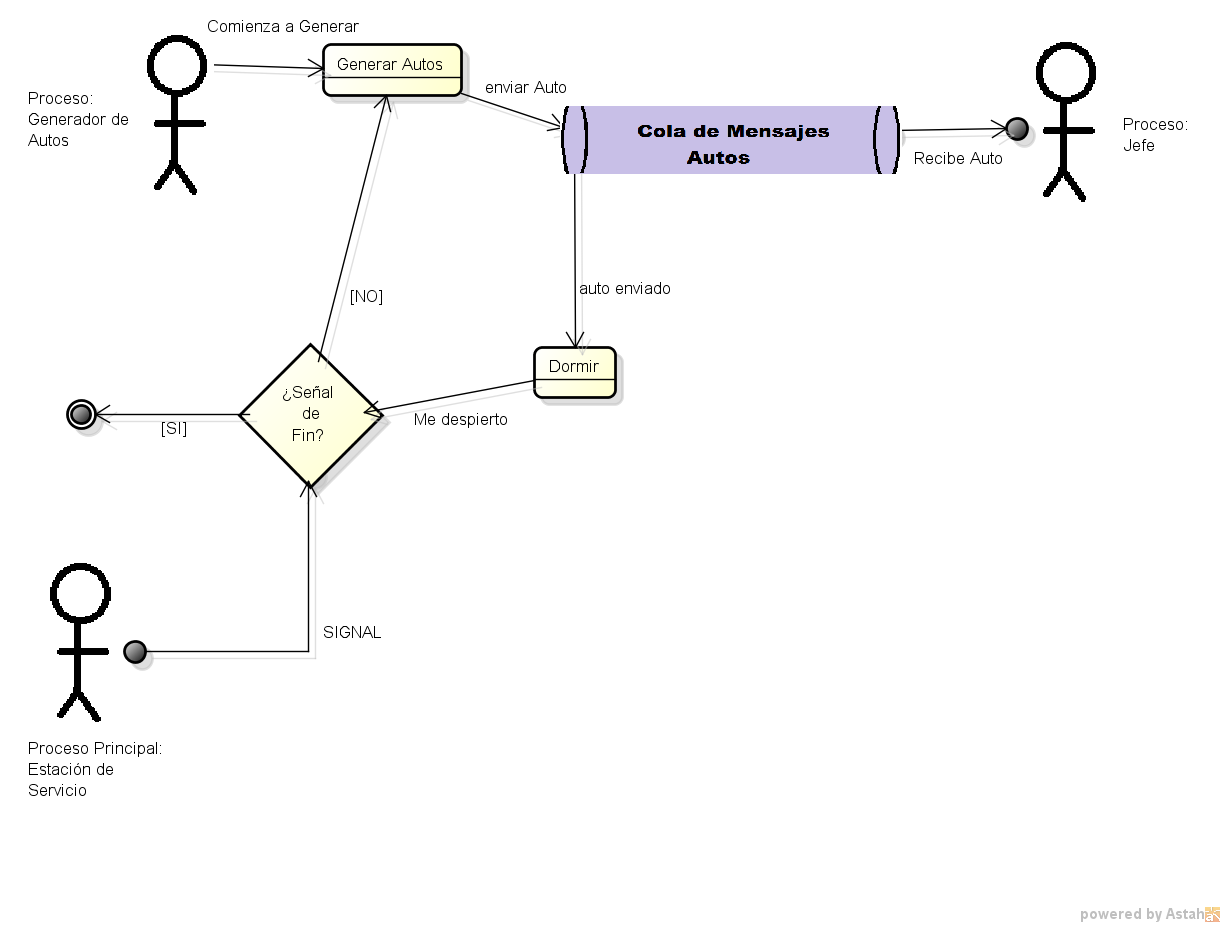
\includegraphics[scale=0.55]{Diagramas/GeneradorDeAutos.png} 
\caption{Diagrama de Funcionamiento y Comunicación de Generador de Autos}
\label{fig:GeneradorDeAutos}
\end{figure}	

\begin{figure}
\centering
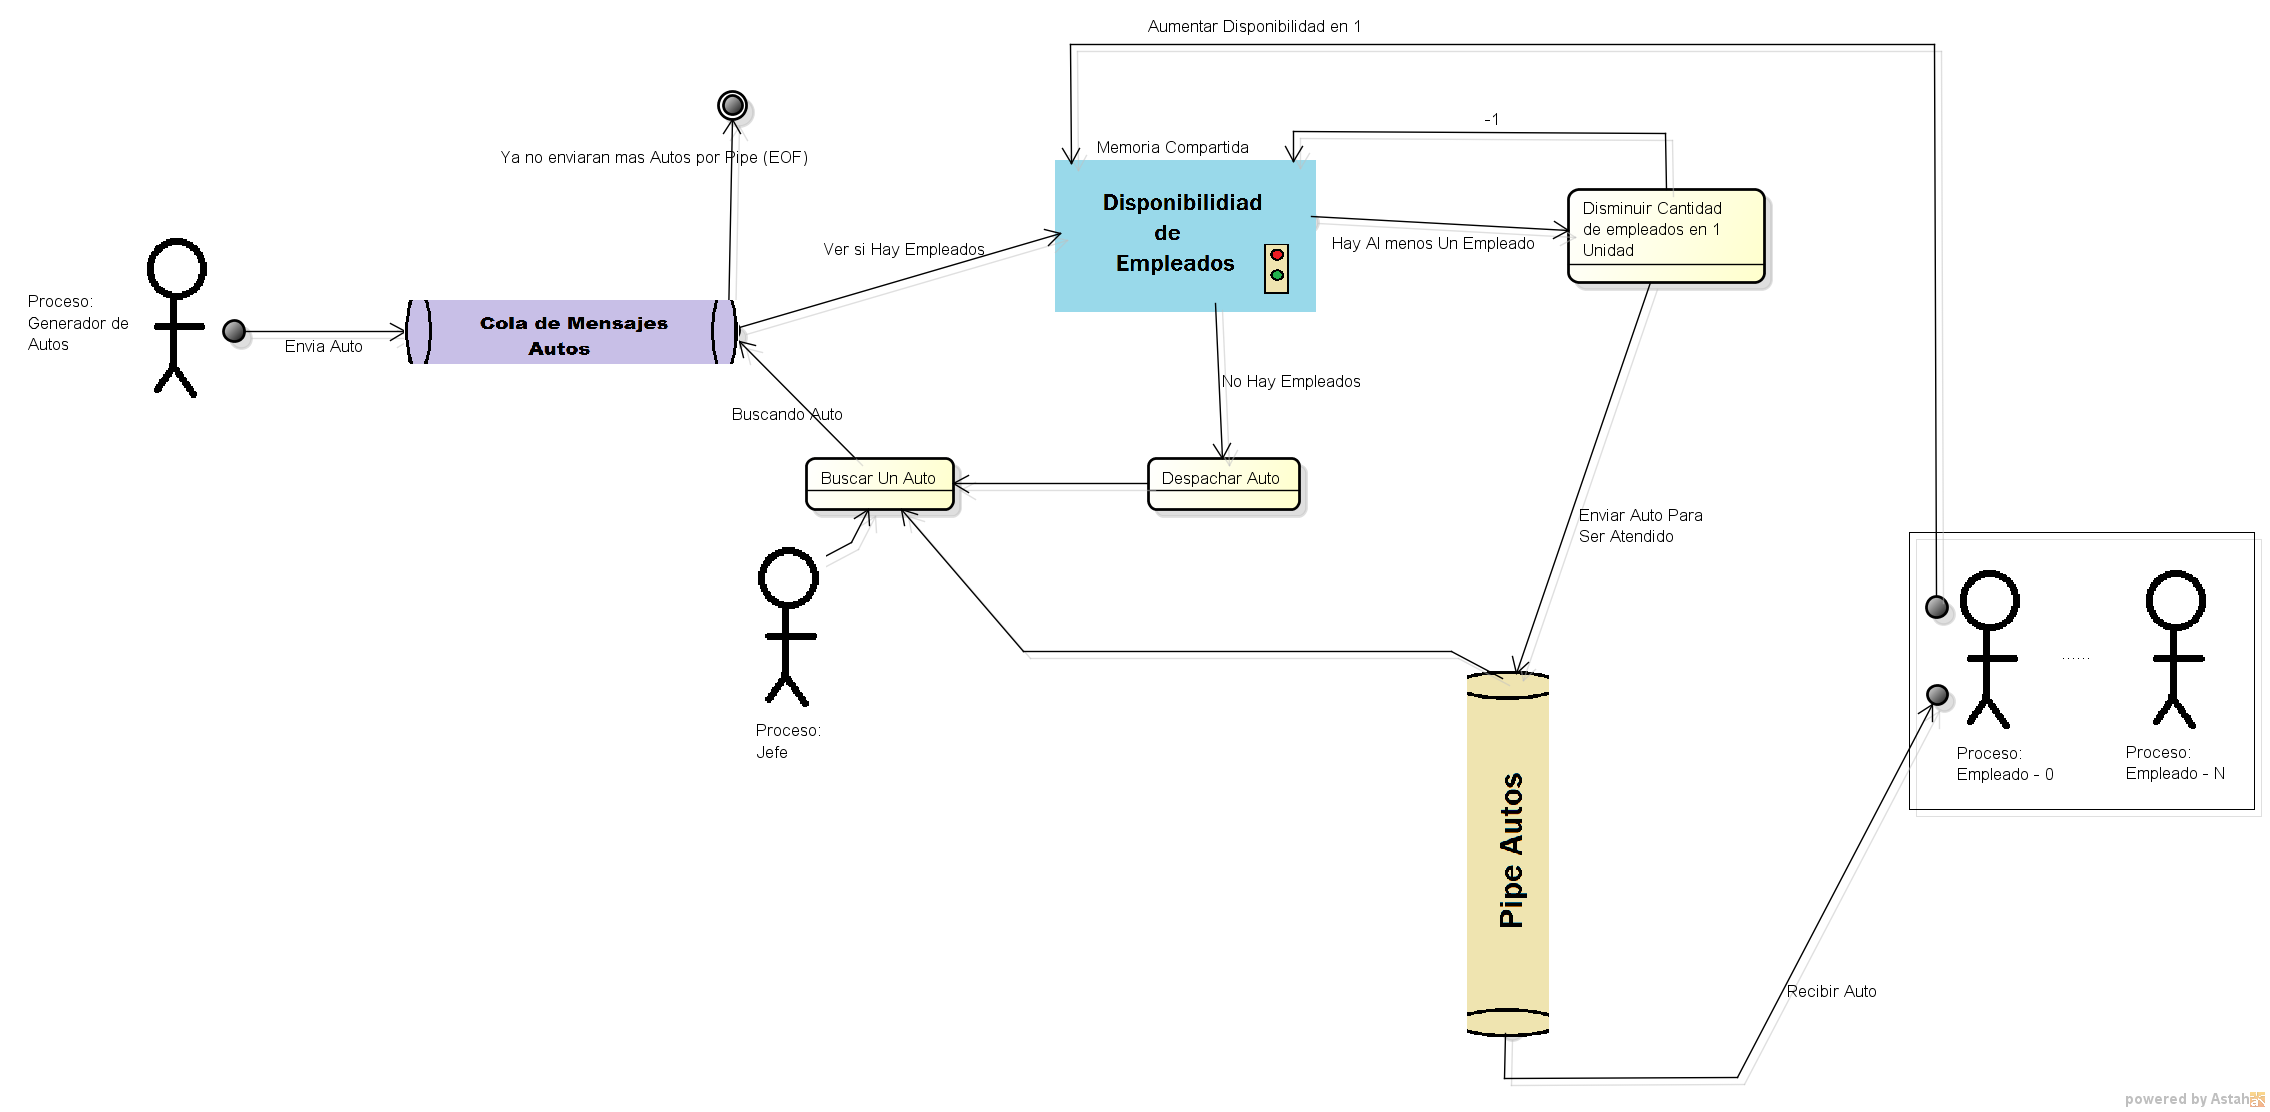
\includegraphics[scale=0.3]{Diagramas/Jefe.png}
\caption{Diagrama de Funcionamiento y Comunicación del Jefe}
\label{fig:Jefe}
\end{figure}	

\begin{figure}
\centering
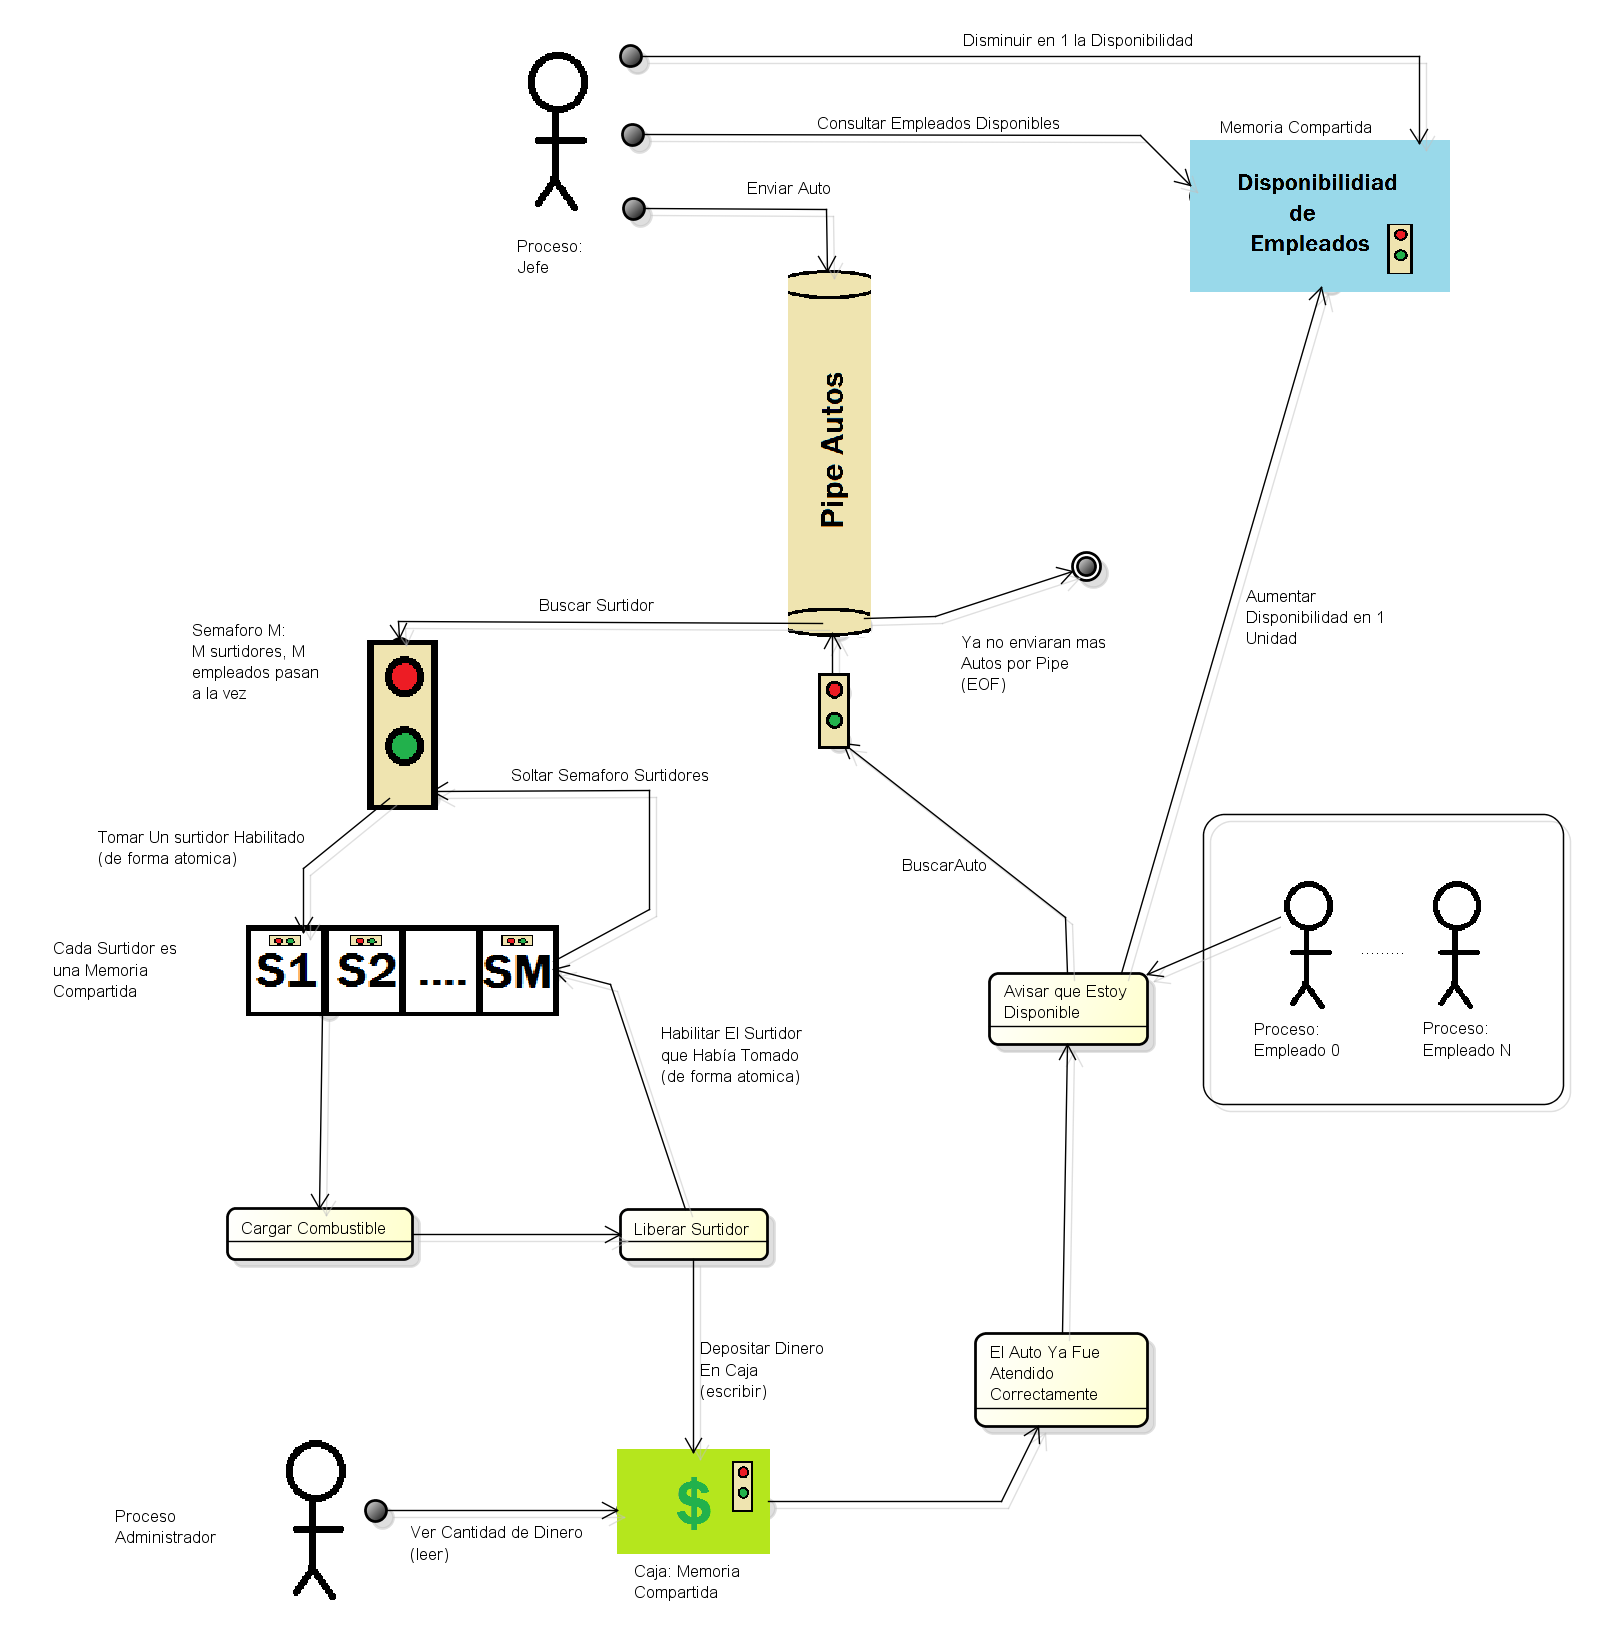
\includegraphics[scale=0.4]{Diagramas/empleados.png}
\caption{Diagrama de Funcionamiento y Comunicación de Empleados}
\label{fig:Empleados}
\end{figure}

\begin{figure}
\centering
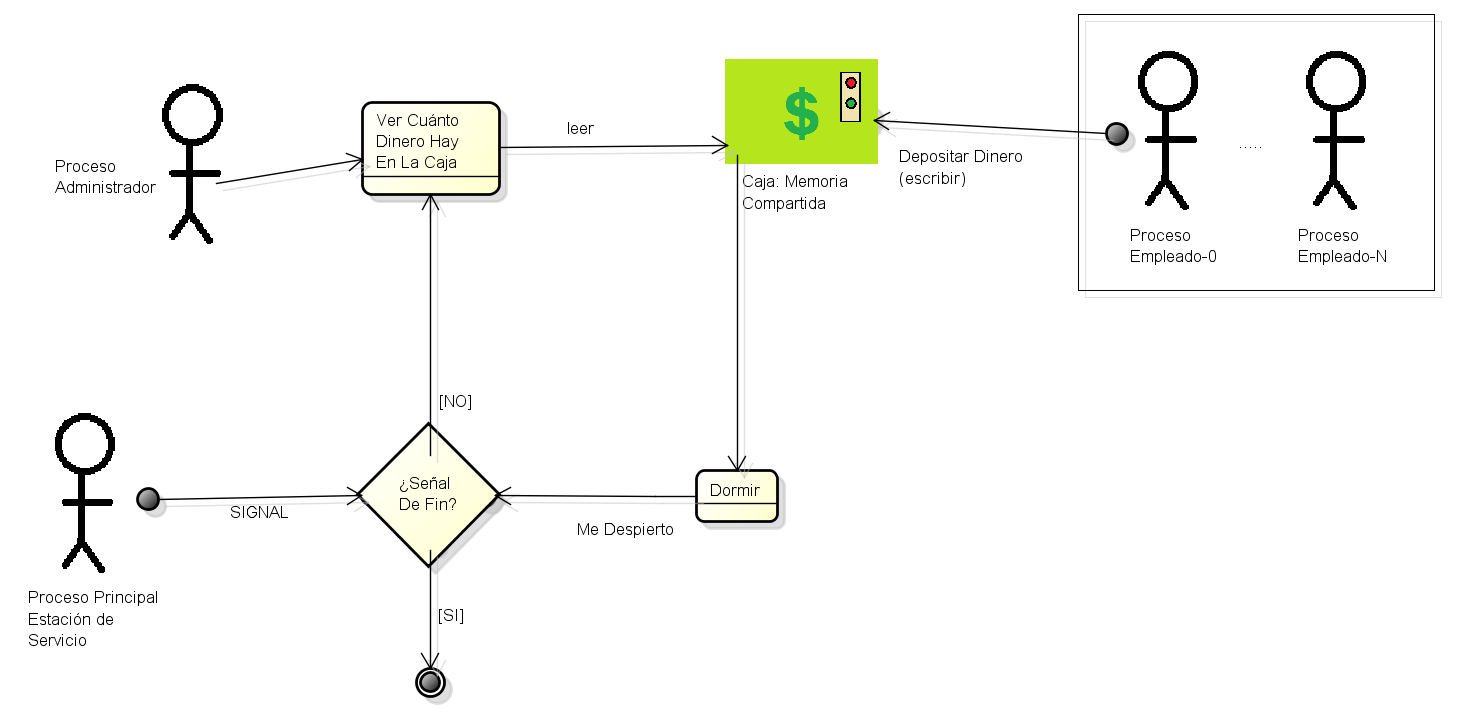
\includegraphics[scale=0.45]{Diagramas/administrador.png}   
\caption{Diagrama de Funcionamiento y Comunicación del Administrador}
\label{fig:Administrador}
\end{figure}

\newpage

	Para la escritura del archivo de Log, se optó por tener un archivo en el que cada proceso pueda escribir haciendo uso de Locks. Cuando un proceso quiere escribir una entrada en el log, intenta tomar el Lock, escribe y luego lo libera. De esta manera, no se corre riesgos de que más de un proceso esté escribiendo en el archivo al mismo tiempo.

\begin{figure}[h!]
\centering
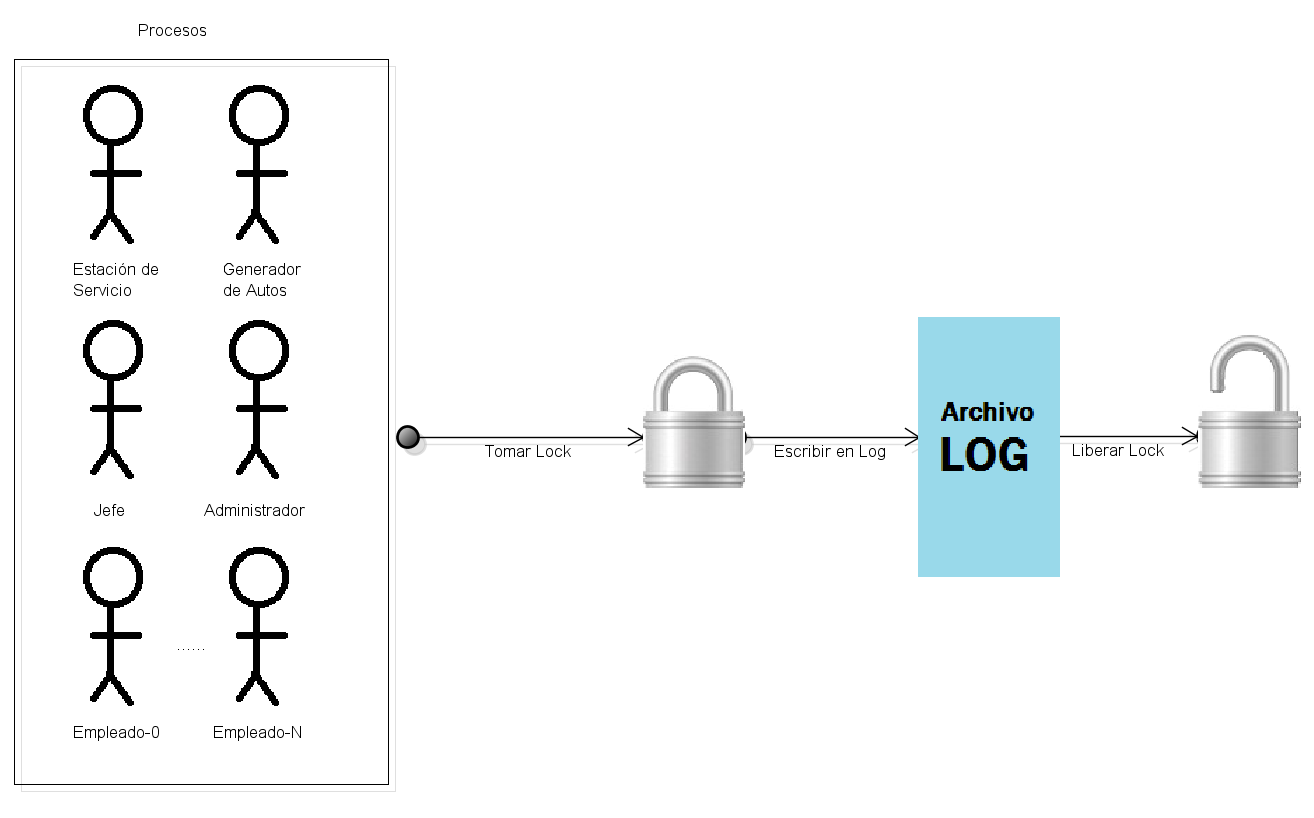
\includegraphics[scale=0.4]{Diagramas/Log.png} 
\caption{Comunicación con el Log}
\label{fig:Log}
\end{figure}	

\newpage

\section{Diagrama de Clases}

\begin{figure}[h!]
\centering
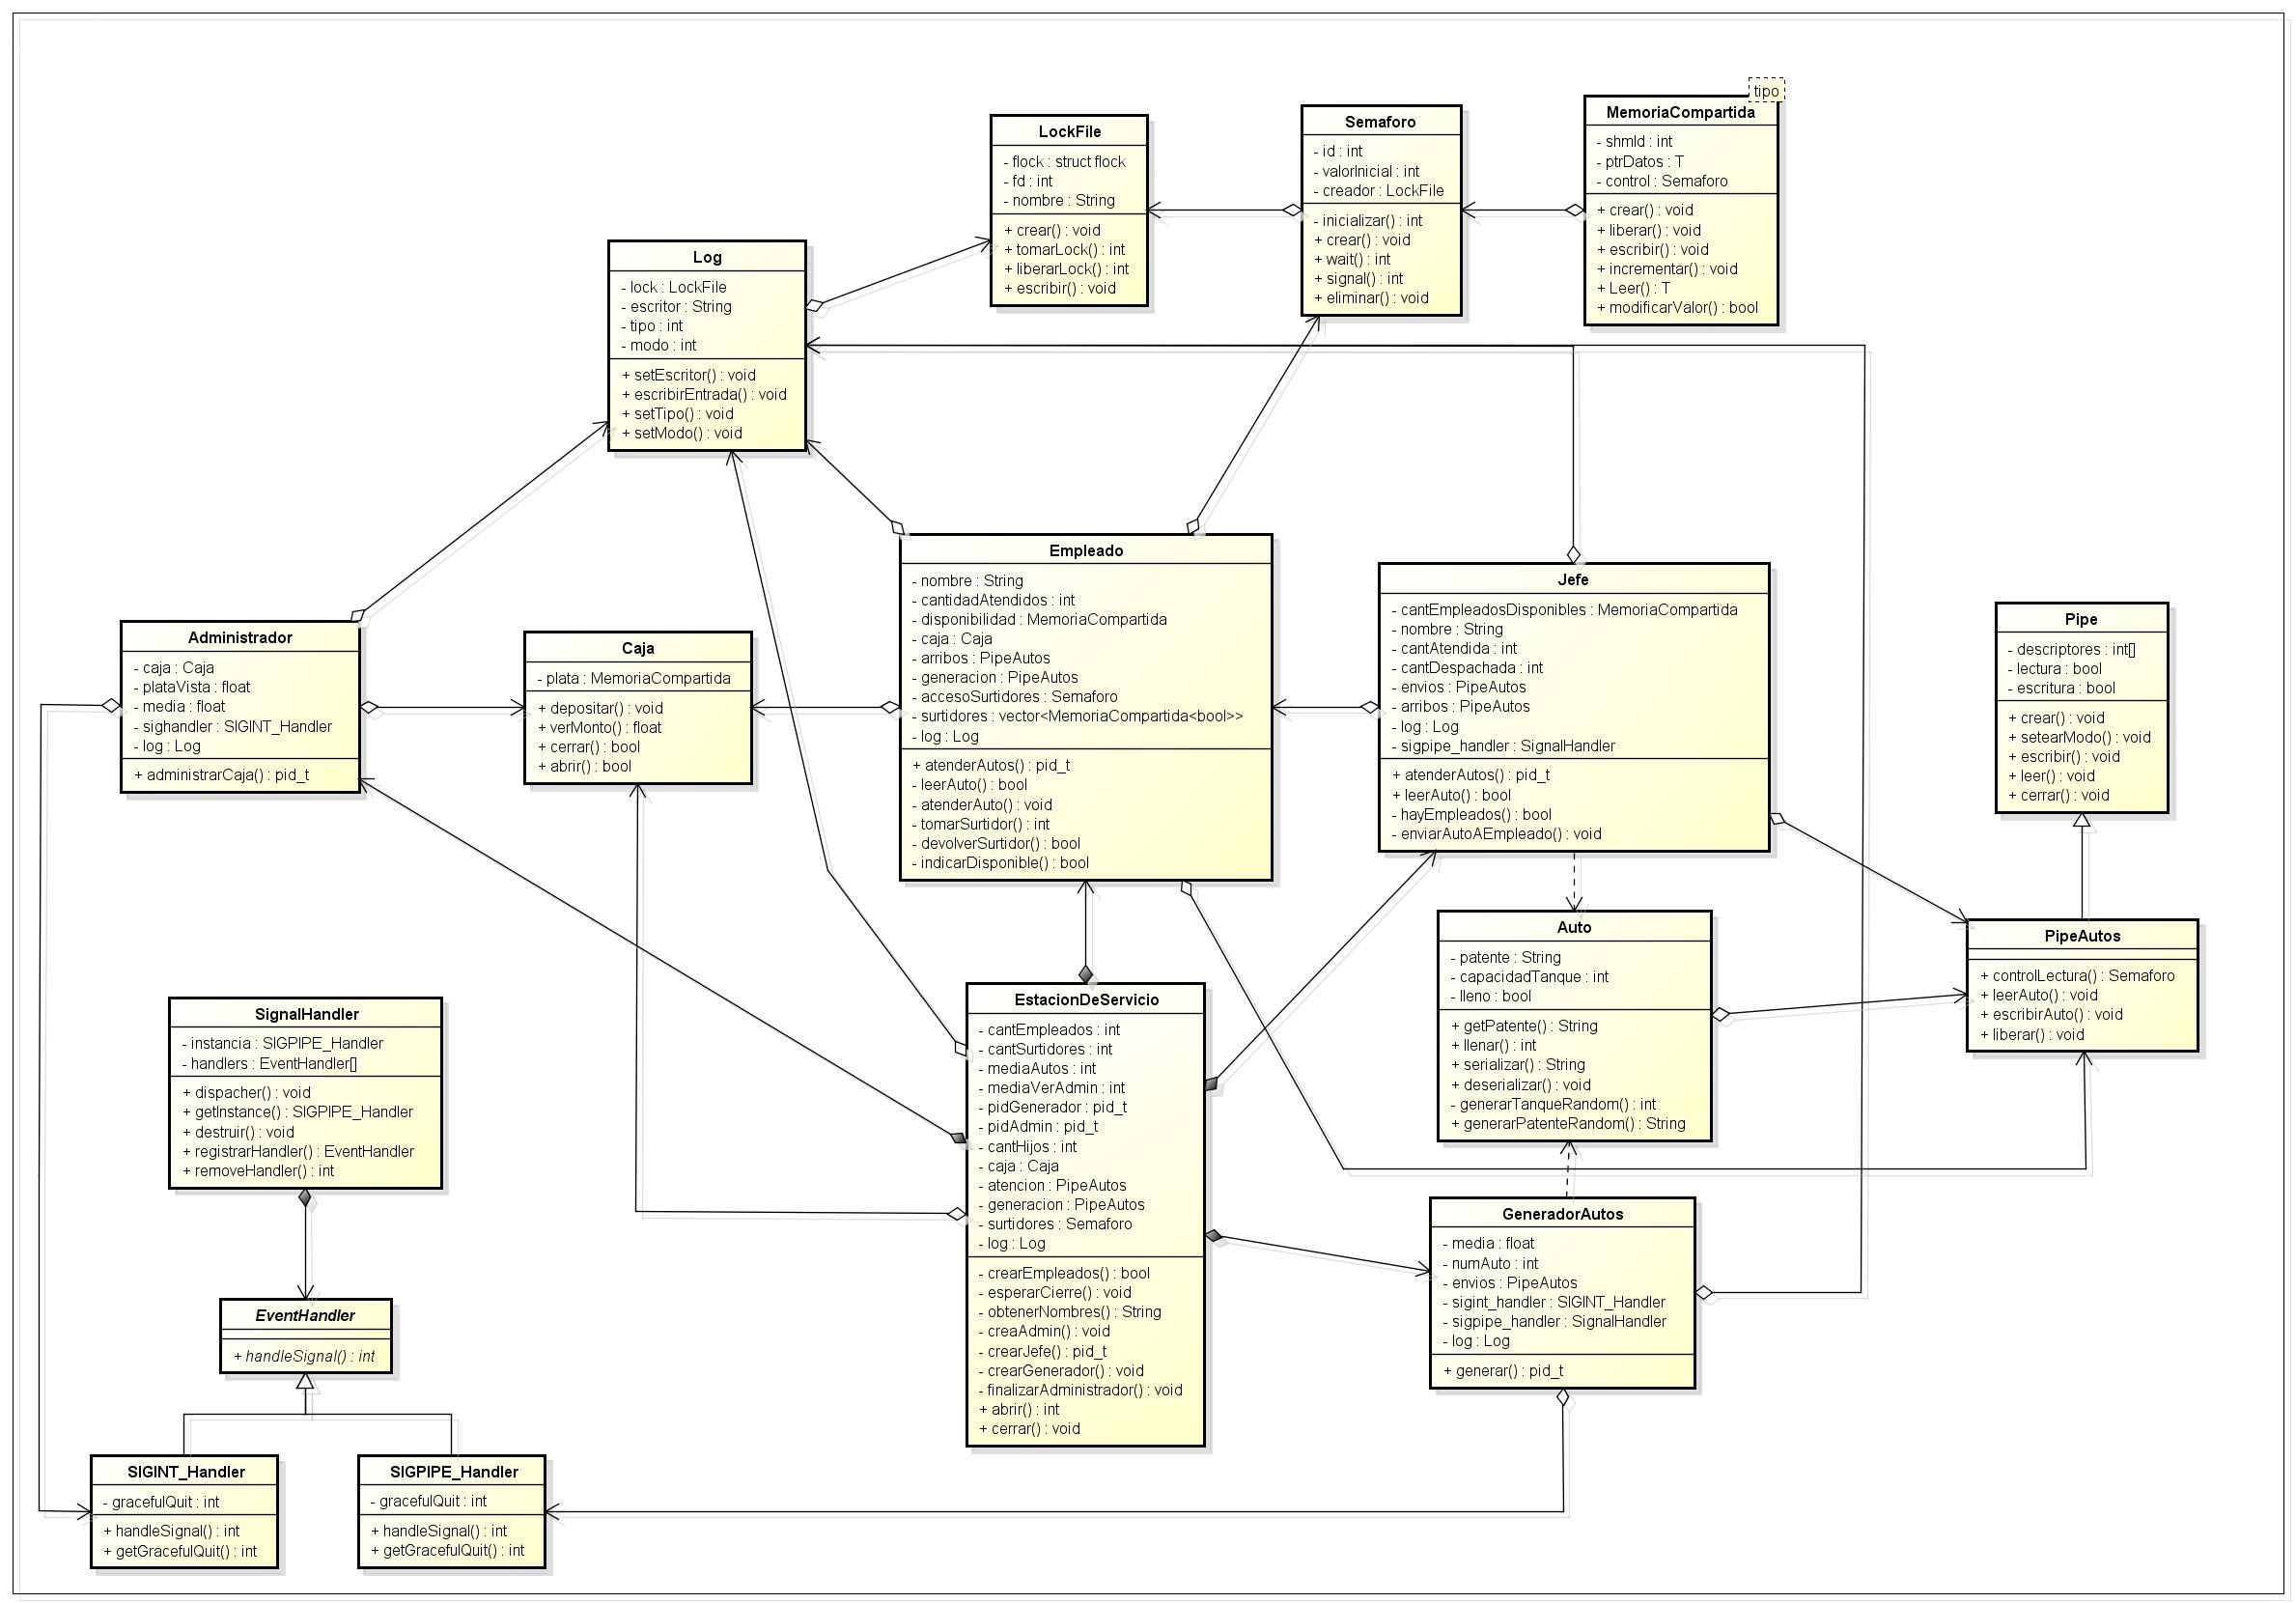
\includegraphics[scale=0.33, angle=90]{Diagramas/clases.jpg} 
\caption{Diagrama de Clases}
\end{figure}

\newpage
\section{Diagramas de Transición de Estados del Jefe}

\begin{figure}[h!]
\centering
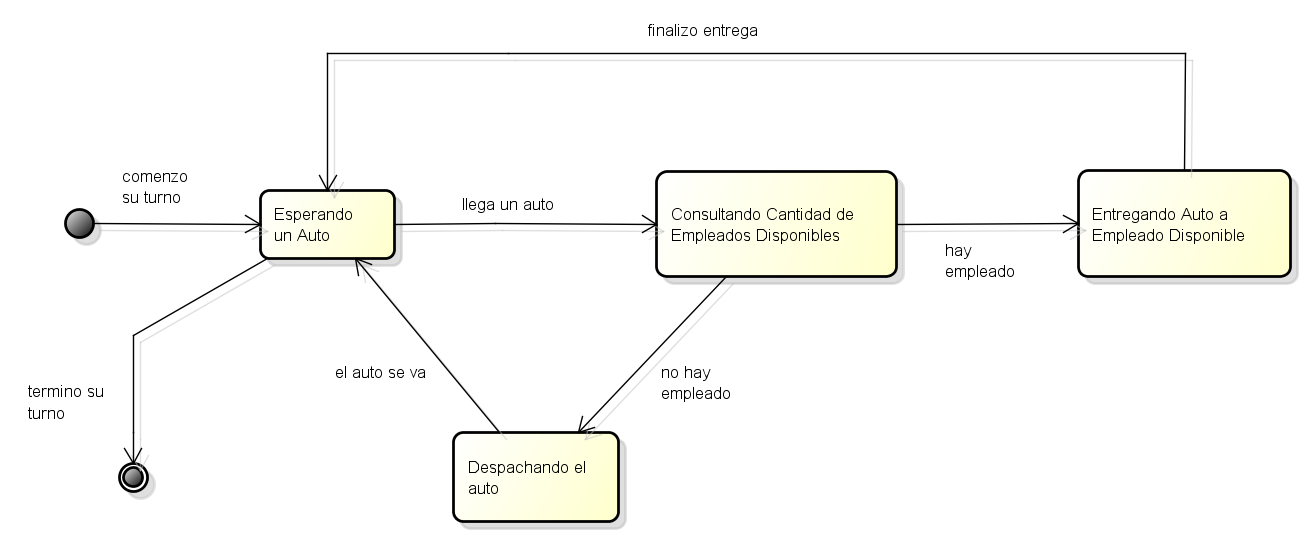
\includegraphics[scale=0.5]{Diagramas/DiagramaDeEstadosJefe.png} 
\caption{Diagrama de Transición de Estados Jefe}
\label{fig:DiagramaDeEstadosJefe}
\end{figure}	


\end{document}